%%==================================================
%% chapter02.tex for SJTU Master Thesis
%% Encoding: UTF-8
%%==================================================

\chapter{Trivium流密码算法}

\section{标准的Trivium流密码算法}

由Christophe De 和 Bart Preneel设计的标准Trivium算法共有288个内部状态位,这288位内部状态的每一次更新构成了Trivium算法生成密钥流中一位密钥的生成来源, Trivium算法的具体应用步骤如下:

\begin{enumerate}[label=(\arabic*),noitemsep,topsep=0pt,parsep=0pt,partopsep=0pt]
  \item 密钥分配阶段:用户通过事先定义或者协商得到密钥K和初始向量IV。
  \item 初始化阶段:将密钥K和初始向量IV装填入Trivium的288位的内部状态中,并运行几轮Trivium算法更新内部状态。
  \item 密钥流生成阶段:每运行一轮Trivium,更新内部状态并生成一位密钥输出。
\end{enumerate}

下面对每个阶段的具体步骤进行详细描述。

\subsection{Trivium算法内部状态的初始化}

Trivium算法内部状态的初始化,可以用以下步骤描述:

\begin{enumerate}[label=(\arabic*),noitemsep,topsep=0pt,parsep=0pt,partopsep=0pt]
  \item 将Trivium的内部状态分为3个部分,第一部位为1到93位,第二部分为94到177位,第三部分为178到288位。
  \item 将80比特的密钥装填入第一部分的前80位即1到80位,并将第一部分的其他位置0,即81到93位置0。
  \item 将80比特的初始向量装填入第二部分的前80位即94到173位,并将第二部分的其他位置0,即174到177位置0。
  \item 将第三部分的后3位置1,即286到288位置1,并将第三部分的其他位置0,即178到285位置0。
  \item 运行 4*288=1152 轮Trivium算法更新内部状态。
\end{enumerate}

可以使用伪代码算法\ref{algo:trivium_intialize}表示这个过程:

\begin{algorithm}[H]
\caption{Trivium算法内部状态初始化过程}
\label{algo:trivium_intialize}
\begin{algorithmic}

  \STATE {$(S_{1}, S_{2},\ldots, S_{93}) \leftarrow (K_{1}, K_{2}, \ldots, K_{80}, 0, \ldots, 0)$}
  \STATE {$(S_{94}, S_{2},\ldots, S_{177}) \leftarrow (IV_{1}, IV_{2}, \ldots, IV_{80}, 0, \ldots, 0)$}
  \STATE {$(S_{178}, S_{2},\ldots, S_{288}) \leftarrow (0, \ldots, 0, 1, 1, 1)$}
  \FOR {$i \leftarrow 1$ \TO $1152$}
    \STATE {$T_{1} \leftarrow S_{66} + S_{93} + S_{91} * S_{92} + S_{171}$}
    \STATE {$T_{2} \leftarrow S_{162} + S_{177} + S_{175} * S_{174} + S_{264}$}
    \STATE {$T_{3} \leftarrow S_{243} + S_{288} + S_{286} * S_{287} + S_{69}$}
    \FOR {$j \leftarrow 2 $\TO $288$}
     \STATE {$S_{j} \leftarrow S_{j-1}$}
    \ENDFOR
    \STATE {$S_{1} \leftarrow T_{3}$}
    \STATE {$S_{94} \leftarrow T_{1}$}
    \STATE {$S_{178} \leftarrow T_{2}$}
  \ENDFOR

\end{algorithmic}
\end{algorithm}



\subsection{Trivium算法密钥流的生成}
Trivium算法的密钥流生成的过程与Trivium算法的初始化过程基本是完全一致的,唯一的区别在于除了要更新Trivium的内部状态之外,每轮还需要使用6位内部状态位来生成密钥比特。

可以使用伪代码算法\ref{algo:trivium_generate}表示这个过程:

\begin{algorithm}[H]
\caption{Trivium算法密钥流的生成过程}
\label{algo:trivium_generate}
\begin{algorithmic}
  \FOR {$i \leftarrow 1$ \TO $N$}
    \STATE {$R_{1} \leftarrow S_{66} + S_{93}$}
    \STATE {$R_{2} \leftarrow S_{162} + S_{177}$}
    \STATE {$R_{3} \leftarrow S_{243} + S_{288}$}
    \STATE {$Z \leftarrow R_{1} + R_{2} + R_{3}$}
    \STATE {$T_{1} \leftarrow R_{1} + S_{91} * S_{92} + S_{171}$}
    \STATE {$T_{2} \leftarrow R_{2} + S_{175} * S_{174} + S_{264}$}
    \STATE {$T_{3} \leftarrow R_{3} + S_{286} * S_{287} + S_{69}$}
    \FOR {$j \leftarrow 2 $\TO $288$}
     \STATE {$S_{j} \leftarrow S_{j-1}$}
    \ENDFOR
    \STATE {$S_{1} \leftarrow T_{3}$}
    \STATE {$S_{94} \leftarrow T_{1}$}
    \STATE {$S_{178} \leftarrow T_{2}$}
  \ENDFOR
\end{algorithmic}
\end{algorithm}


\subsection{Trivium算法的硬件实现}

\begin{figure}[H]
	\centering
	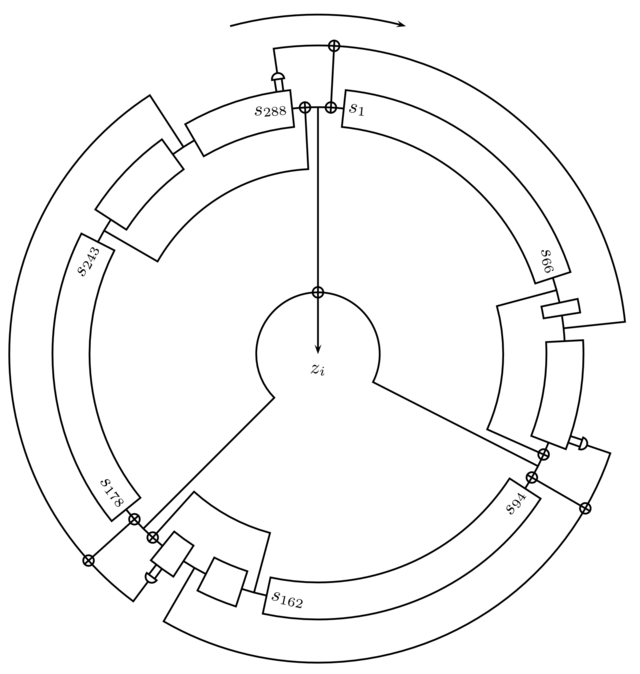
\includegraphics[width=0.5\textwidth]{chap2/hardwareTrivium.png}
	\caption{Trivium算法的硬件实现}\label{fig:Trivium算法的硬件实现}
\end{figure}

如图\ref{fig:Trivium算法的硬件实现}所示,Trivium的硬件实现包含了288个移位寄存器以及3个与门11个异或门。一个移位寄存器约需7个逻辑门实现,这样,Trivium算法的硬件实现需约2030个逻辑门,而如果全部使用与或门来实现,则约需3000个逻辑门。

\section{Trivium算法的结构}

传统的流密码算法仅有线性反馈移位寄存器实现,因此传统的流密码算法都可以将其表示为一个状态转移矩阵的形式,即存在状态转移矩阵A使$(s_{1}, s_{2}, \ldots, s_{n})^{T}$ = $A_{n*n}$ * $(s_{1}, s_{2}, \ldots, s_{n})^{T}$,然后将状态转移矩阵转化为一个特征多项式进行研究,而Trivium算法除了传统的线性反馈移位寄存器外,还含有三个非线性反馈移位寄存器,因此很难找到一个简单合适的方法将其表示成一个状态转移矩阵或者特征多项式,为了研究方便,本节将先从Trivium算法的线性部分研究Trivium算法的线性部分的结构。

\subsection{Trivium算法的线性部分的状态转移矩阵}

对于仅基于线性反馈移位寄存器的流密码,将其表述成一个状态转移矩阵是一件简单的事,并且通过状态转移矩阵或通过状态转移矩阵得到的特征多项式可以有效地分析密码的性质。虽然Trivium算法包含非线性反馈移位寄存器的部分,但在算法\ref{algo:trivium_intialize}中可以发现$S_{66} + S_{93} + S_{91} * S_{92} + S_{171}$、$S_{162} + S_{177} + S_{175} * S_{174} + S_{264}$、$S_{243} + S_{288} + S_{286} * S_{287} + S_{69}$是Trivium算法中的主要部分,且可以拆成线性部分和非线性部分的组合,形成如$(s_{1}, s_{2}, \ldots, s_{n})^{T}$ = $A_{n*n}$ * $(s_{1}, s_{2}, \ldots, s_{n})^{T}$ + $(w_{1}, w_{2}, \ldots, w_{n})^{T}$的形式。

对于Trivium算法的线性部分,我们可以得到如下方程:

令
\begin{align}
\label{eq:struct_A}
& A = \left(
\begin{array}{@{}*{6}{c}@{}}
0 & 0 & 0 & \cdots & 0 & 1 \\
1 & 0 & 0 & \cdots & 0 & 0 \\
0 & 1 & 0 & \cdots & 0 & 0 \\
\vdots & & \ddots & & & \vdots \\
\vdots & & & \ddots & & \vdots \\
0 & 0 & 0 & \cdots & 1 & 0 \\
\end{array}
\right)+\left(
\begin{array}{@{}*{9}{c}@{}}
0 & \cdots & 1_{(1,69)} & \cdots & 0 & \cdots & 1_{(1,243)} & \cdots & 0 \\
0 & \cdots & \cdots & \cdots & 0 & \cdots & \cdots & \cdots & 0 \\
\vdots & & & & & & & & \vdots \\
0 & \cdots & 1_{(94,66)} & \cdots & 0 & \cdots & 1_{(94,171)} & \cdots & 0 \\
\vdots & & & & & & & & \vdots \\
0 & \cdots & \cdots & 1_{(178,162)}  & \cdots & \cdots & 1_{(178,264)} & \cdots & 0 \\
\vdots & & & & & & & & \vdots \\
0 & \cdots & \cdots & \cdots & 0 & \cdots & \cdots & \cdots & 0 \\
\end{array}
\right)
\end{align}

\begin{align}
\label{eq:struct_S}
& S = \left(
\begin{array}{@{}*{6}{c}@{}}
S_{1} \\
S_{2} \\
\vdots \\
S_{288} \\
\end{array}
\right)
\end{align}

\begin{align}
\label{eq:struct_C}
& C = \left(
\begin{array}{@{}*{6}{c}@{}}
S_{226} * S_{227} \\
\vdots \\
S_{91} * S_{92} \\
\vdots \\
S_{175} * S_{176} \\
\vdots \\
0 \\
\end{array}
\right)
\end{align}

从而有:
\begin{align}
\label{eq:struct}
& S = A \cdot S + C
\end{align}

从上述的的一系列的等式中,A是状态转移的线性部分,C是非线性部分,S是288位移位寄存器,A赋值等式右边的第一项代表了Trivium算法的位移过程,而A赋值等式右边的第二项代表了Trivium算法的替换更新过程。

\subsection{Trivium型算法的定义}

\subsubsection{Trivium算法的线性部分的状态转移矩阵的特征多项式}

进一步研究Trivium算法的线性部分的状态转移矩阵即A,首先可以计算在模2域上状态转移矩阵A所对应的特征多项式,由状态转移矩阵计算特征多项式的方法为计算|A-xI|的值,其中I为单位矩阵。

计算状态转移矩阵A所对应的特征多项式可分为手工计算和程序实现两种方案。首先介绍手工计算的大致思路,首先如果忽略线性部分中$S_{66} + S_{171}$、$S_{162} + S_{264}$、$S_{243} + S_{69}$这三部分,那么很容易得知此时的状态转移矩阵A除了所有$A_{(i,i-1)}$(包括$A_{(1,288)}$)为1外,其他全部为0,此时可以较轻易计算出状态转移矩阵对应的特征多项式。同时,可以注意到忽略的三部分,其实影响的仅为状态转移矩阵中的6位,即仍有6位需要置1,此时可以通过逐渐将这6个1填回状态转移矩阵中,然后通过矩阵的分解展开逐步计算每次添加1个1后新的状态转移矩阵对应的特征多项式。

可见上述方法计算起来十分复杂,并且要将这种方法转为通用的计算程序也并不容易。因此本文著者在研究中采用通过以下Maple程序代码(算法\ref{algo:trivium_maple_function}),计算Trivium算法对应的状态转移矩阵A并计算该状态转移矩阵A对应的特征多项式:

\begin{algorithm}[H]
  \caption{Maple计算特征多项式}
  \label{algo:trivium_maple_function}
  \begin{algorithmic}
      
	  \STATE {$(w_{1}, w_{2}, \ldots, w_{9}) \leftarrow (22, 23, 31, 54, 57, 59, 81, 88, 96)$}
	  \STATE $A \leftarrow Matrix(w_{9}*3)$
	  \STATE $A[1][w_{9}*3] \leftarrow 1$
	  \FOR {$i \leftarrow 2$ \TO $(w_{9} * 3)$}
	    \STATE $A[i][i - 1] \leftarrow 1$
	  \ENDFOR 
	  \STATE $A[3*w_{3}+1][3*w_{1}] \leftarrow 1$
	  \STATE $A[3*w_{3}+1][3*w_{5}] \leftarrow 1$
	  \STATE $A[3*w_{6}+1][3*w_{4}] \leftarrow 1$
	  \STATE $A[3*w_{6}+1][3*w_{8}] \leftarrow 1$
	  \STATE $A[1][3*w_{2}] \leftarrow 1$
	  \STATE $A[1][3*w_{7}] \leftarrow 1$
	  \STATE $f \leftarrow charpoly(A, x) mod \quad 2$

  \end{algorithmic}
\end{algorithm}

Maple计算得到的结果可以得到Trivium算法的特征多项式为

\[\begin{split}
f(x)&=x^{288}+x^{219}+x^{210}+x^{201}+x^{141}+x^{132}+x^{123}\\
&+x^{87}+x^{72}+x^{60}+x^{54}+x^{45}+x^{42}+x^{27}+x^{15}+1\\
\end{split}\]
\begin{equation}
\label{eq:feature_polynom}
\end{equation}

\subsubsection{Trivium算法的特征多项式中的$(x+1)^3$因子}

在计算出Trivium算法线性部分对应的状态转移矩阵的特征多项式后,我们继续深入研究式(\ref{eq:feature_polynom})的整除性,为之后引入Trivium型算法做准备。

\begin{algorithm}[H]
  \caption{Maple验证整除性}
  \label{algo:maple_divide}
  \begin{algorithmic}
      
	   \STATE $f \leftarrow x^{288}+x^{219}+x^{210}+x^{201}+x^{141}+x^{132}+x^{123}+x^{87}+x^{72}+x^{60}+x^{54}+x^{45}+x^{42}+x^{27}+x^{15}+1$
       \STATE $Divide(f,(x+1)^{3},'g') mod \quad 2$

  \end{algorithmic}
\end{algorithm}

由上述代码的结果可以发现$(x+1)^3|f(x)$。


进一步分析特征多项式的特点,还能得到一个更强的结论。

\begin{algorithm}[H]
  \caption{Maple验证整除性的更强结论}
  \label{algo:maple_divide_2}
  \begin{algorithmic}
      
	   \STATE $f \leftarrow x^{288}+x^{219}+x^{210}+x^{201}+x^{141}+x^{132}+x^{123}+x^{87}+x^{72}+x^{60}+x^{54}+x^{45}+x^{42}+x^{27}+x^{15}+1$
       \STATE $Divide(f,(x^{3}+1)^{3},'g') mod \quad 2$

  \end{algorithmic}
\end{algorithm}

由上述代码的结果可以发现$(x^3+1)^3|f(x)$。

\subsubsection{Trivium算法的特征多项式中的本原多项式}

从上述对Trivium算法的整数性分析,可以发现标准Trivium算法的特征多项式可以在模2域上因式分解,并可以得到下列等式:
\[\begin{split}
\frac{f(x)}{(x^3+1)^3}=&x^{279}+x^{276}+x^{267}+x^{264}+x^{255}+x^{252}+x^{243}\\
&+x^{240}+x^{231}+x^{228}+x^{219}+x^{216}+x^{210}+x^{204}+x^{201}+x^{132}+x^{129}\\
&+x^{123}+x^{117}+x^{114}+x^{105}+x^{102}+x^{93}+x^{90}+x^{81}+x^{75}+x^{69}+x^{60}\\
&+x^{57}+x^{51}+x^{42}+x^{39}+x^{36}+x^{27}+x^{24}+x^{18}+x^{12}+x^3+1\\
f(x)=&(x^3+1)^3g(x^3)
\end{split}\]
\begin{equation}
\label{eq:trivium_expand}
\end{equation}

式(\ref{eq:trivium_expand})中g(x)为GF(2)上的93次本原多项式。由此我们可以将Trivium算法参数化并给出Trivium型算法的定义:
\begin{defn}[Trivium型算法的定义]
\label{defn:trivium}

算法形如(\ref{algo:trivium_generate_param})

\begin{algorithm}[H]
\caption{Trivium型算法}
\label{algo:trivium_generate_param}
\begin{algorithmic}
  \FOR {$i \leftarrow 1$ \TO $N$}
    \STATE {$R_{1} \leftarrow S_{3*\omega[1]} + S_{3*\omega[3]}$}
    \STATE {$R_{2} \leftarrow S_{3*\omega[4]} + S_{3*\omega[6]}$}
    \STATE {$R_{3} \leftarrow S_{3*\omega[7]} + S_{3*\omega[9]}$}
    \STATE {$Z \leftarrow R_{1} + R_{2} + R_{3}$}
    \STATE {$T_{1} \leftarrow R_{1} + S_{3*\omega[3]-2} * S_{3*\omega[3]-1} + S_{3*\omega[5]}$}
    \STATE {$T_{2} \leftarrow R_{2} + S_{3*\omega[6]-2} * S_{3*\omega[6]-1} + S_{3*\omega[8]}$}
    \STATE {$T_{3} \leftarrow R_{3} + S_{3*\omega[9]-2} * S_{3*\omega[9]-1} + S_{3*\omega[2]}$}
    \FOR {$j \leftarrow 2 $\TO $3*\omega[9]$}
     \STATE {$S_{j} \leftarrow S_{j-1}$}
    \ENDFOR
    \STATE {$S_{1} \leftarrow T_{3}$}
    \STATE {$S_{3*\omega[3]+1} \leftarrow T_{1}$}
    \STATE {$S_{3*\omega[6]+1} \leftarrow T_{2}$}
  \ENDFOR
\end{algorithmic}
\end{algorithm}

其中$\omega = (\omega[1], \omega[2], \ldots, \omega[9])$,且$\omega[1] < \omega[2] < \ldots < \omega[9]$,共$3*\omega[9]$位内部状态,由此得到的线性部分对应的状态转移矩阵的特征多项式为f(x),如果f(x)可表示为$(x^{3}+1)^{3}g(x^{3})$的形式,并且g(x)为模2域上的本原多项式,那么定义这个算法为Trivium型算法。

\end{defn}

\subsection{n阶Trivium型算法}

考虑到标准Trivium算法存在一个弱化算法Bivium,Bivium和Trivium的区别在于Trivium是一个3轮的算法,即从硬件的角度看Trivium的内部状态被切割为3段,而Bivium的内部状态是2段。因此在Trivium型算法的基础上再次进行扩展,形成n阶Trivium型算法的概念,即从硬件角度看内部状态被分割为n段,从算法实现角度看,由原来的9个参数变为3n个参数,并且此时需要特征多项式f(x)能整除$(x+1)^{n}$且整除后的商是一个本原多项式。

\section{Trvium算法的安全性}
根据Trvium型算法的定义(\ref{defn:trivium}),可知本原多项式是Trivium算法的安全基础,正是由于本原多项式使得Trivium算法在理论上的线性部分的周期很大,然后Trivium算法作者声称通过引入非线性部分,周期总是能大于线性部分周期以此保证Trivium算法的大周期导致的安全性。因此本节将通过研究Trivium算法的周期考察其安全性。

\subsection{Trivium型算法的本原多项式的最小次数}
标准的Trivium算法建立在式(\ref{eq:trivium_expand})的本原多项式上,该本原多项式的最高次数为93,多项式指数(Polynomial Order)为93,光线性部分的周期就非常大了,因此不便于作深入的分析研究。根据定义(\ref{defn:trivium})可知Trivium型算法可以通过降低本原多项式的次数降低线性部分的周期进而可能降低整体周期,假设已知本原多项式g(x),在保证g(x)的最高次数尽可能低的前提下,计算$f(x)=(x^{3}+1)^{3}g(x^{3})$,然后通过f(x)还原出除$A_{(i,i-1)}$外仅有6个位置为1的状态转移矩阵A,再根据状态转移矩阵A求解$\omega_{1},\omega_{2},\cdots,\omega_{9}$,从上述描述就可知直接根据g(x)求解$\omega_{1},\omega_{2},\cdots,\omega_{9}$是非常困难的。但可以反其道而行,通过遍历$\omega_{1},\omega_{2},\cdots,\omega_{9}$,从而推导出对应的特征多项式f(x),然后先检查其能否表示成$f(x)=(x^{3}+1)^{3}g(x^{3})$的形式,如果能再检查g(x)是否是本原多项式,再在其中找出最高次数最低的g(x)是一个可行的方案。在Maple上本文著者通过以下代码运行出了Trivium型算法的最小的本原多项式次数:

\begin{breakablealgorithm}
  \caption{Trivium算法最小阶数计算}
  \label{algo:trivium_maple}
  \begin{algorithmic}
    
    \FOR {$w1 \leftarrow 1$ \TO $6$}
      \FOR {$w2 \leftarrow (w1 + 1)$ \TO $7$}
        \FOR {$w3 \leftarrow (w2 + 1)$ \TO $8$}
          \FOR {$w4 \leftarrow (w3 + 1)$ \TO $9$}
            \FOR {$w5 \leftarrow (w4 + 1)$ \TO $10$}
              \FOR {$w6 \leftarrow (w5 + 1)$ \TO $11$}
                \FOR {$w7 \leftarrow (w6 + 1)$ \TO $12$}
                  \FOR {$w8 \leftarrow (w7 + 1)$ \TO $13$}
                    \FOR {$w9 \leftarrow (w8 + 1)$ \TO $14$}      
                      \STATE {$(w_{1}, w_{2}, \ldots, w_{9}) \leftarrow (w1, w2, \ldots, w9)$}
                      \STATE $A \leftarrow Matrix(w_{9}*3)$
                      \STATE $A[1][w_{9}*3] \leftarrow 1$
                      \FOR {$i \leftarrow 2$ \TO $(w_{9} * 3)$}
                        \STATE $A[i][i - 1] \leftarrow 1$
                      \ENDFOR 
                      \STATE $A[3*w_{3}+1][3*w_{1}] \leftarrow 1$
                      \STATE $A[3*w_{3}+1][3*w_{5}] \leftarrow 1$
                      \STATE $A[3*w_{6}+1][3*w_{4}] \leftarrow 1$
                      \STATE $A[3*w_{6}+1][3*w_{8}] \leftarrow 1$
                      \STATE $A[1][3*w_{2}] \leftarrow 1$
                      \STATE $A[1][3*w_{7}] \leftarrow 1$
                      \STATE $f \leftarrow charpoly(A, x) mod \quad 2$
                      \IF {$Divide(f,(x^{3}+1)^{3},'g') mod \quad 2$}
                        \STATE $g \leftarrow algsubs(x^{3}=x, g)$
                        \IF {$Primitive(g) mod \quad 2$}
                          \STATE $output(w)$
                        \ENDIF
                      \ENDIF
                    \ENDFOR
                  \ENDFOR
                \ENDFOR
              \ENDFOR
            \ENDFOR
          \ENDFOR
        \ENDFOR
      \ENDFOR
    \ENDFOR
    
  \end{algorithmic}
\end{breakablealgorithm}

算法(\ref{algo:trivium_maple})中的9个嵌套的For循环将会遍历1到14中所有的9个参数的取值,由于有$\omega_{1}<\omega_{2}<\cdots<\omega_{9}$这一约束条件,所以其计算量会缩减为$6^9$个处理级别,是一个可以接受的范围,以本文著者普通的笔记本电脑(CPU:i5 2410,内存 4GB)的运算能力运行时间接近1800秒。最后,Maple运算的结果如下表所示:

\begin{table}[H]
  \label{table:trivium_minimal}
  \centering
  \caption{Trivium型算法对应的本原多项式最高次数最小的参数}
  \begin{tabular}{|c|c|}
  	\hline
  	\hline
    $\omega_{1},\omega_{2},\cdots,\omega_{9}$ & 本原多项式 \\ 
	\hline
    1,2,4,5,6,8,9,10,14 & $1+x+x^{4}+x^{7}+x^{9}+x^{10}+x^{11}$ \\
    \hline
    1,2,4,5,6,8,11,13,14 & $1+x+x^{3}+x^{10}+x^{11}$ \\
    \hline
    1,2,4,5,6,10,11,12,14 & $1+x+x^{4}+x^{7}+x^{9}+x^{10}+x^{11}$ \\
    \hline
    1,2,4,6,8,9,11,13,14 & $1+x+x^{3}+x^{4}+x^{7}+x^{8}+x^{9}+x^{10}+x^{11}$ \\
    \hline
    1,2,4,7,9,10,11,12,14 & $1+x+x^{3}+x^{10}+x^{11}$ \\
    \hline
    1,2,6,7,8,10,11,12,14 & $1+x+x^{4}+x^{7}+x^{9}+x^{10}+x^{11}$ \\
    \hline
    1,3,5,6,8,10,12,13,14 & $1+x+x^{2}+x^{3}+x^{4}+x^{7}+x^{8}+x^{10}+x^{11}$ \\
    \hline
    1,3,5,7,8,9,10,12,14 & $1+x+x^{2}+x^{3}+x^{4}+x^{7}+x^{8}+x^{10}+x^{11}$ \\
    \hline
    1,3,6,8,9,10,12,13,14 & $1+x+x^{8}+x^{10}+x^{11}$ \\
    \hline
    2,3,4,5,7,9,10,12,14 & $1+x+x^{2}+x^{3}+x^{4}+x^{7}+x^{8}+x^{10}+x^{11}$ \\
    \hline
    2,3,4,5,7,10,12,13,14 & $1+x+x^{8}+x^{10}+x^{11}$ \\
    \hline
    2,3,4,6,7,8,9,11,14 & $1+x+x^{8}+x^{10}+x^{11}$ \\
    \hline
    2,3,4,6,7,8,12,13,14 & $1+x+x^{2}+x^{4}+x^{7}+x^{10}+x^{11}$ \\
    \hline
    2,3,4,8,9,10,12,13,14 & $1+x+x^{2}+x^{4}+x^{7}+x^{10}+x^{11}$ \\
    \hline
    2,4,5,6,7,9,11,13,14  & $1+x+x^{3}+x^{4}+x^{7}+x^{8}+x^{9}+x^{10}+x^{11}$ \\
    \hline
    2,4,5,7,9,10,11,12,14 & $1+x+x^{3}+x^{4}+x^{7}+x^{8}+x^{9}+x^{10}+x^{11}$ \\
    \hline
    3,5,6,7,8,10,11,12,14 & $1+x+x^{3}+x^{10}+x^{11}$ \\
    \hline
    4,5,6,8,9,10,12,13,14 & $1+x+x^{2}+x^{4}+x^{7}+x^{10}+x^{11}$ \\
    \hline
\end{tabular}
\end{table}

可以看到表(2-1)中,著者列出了满足Trivium型算法的18组参数及其对应计算得到的本原多项式,从表中可知最高阶次数小于11的本原多项式中,并不能反向推出满足Trivium型算法的参数,从而本文著者得到以下结论:
\begin{thm}[Trivium型算法对应的本原多项式最高次数最小为11]
\label{thm:trivium_minimal}
满足定义(\ref{defn:trivium})的所有Trivium型算法中,Min(deg(g(x)))=11,且Trivium型算法内部状态的至少有42位。

定理\ref{thm:trivium_minimal}的证明由表(2-1)可证。
\end{thm}

这个结论说明,Trivium型算法可以通过减少内部状态数量提高效率,然而减少后的内部状态数量仍有限制,且存在下限。

进一步将代码上限由14提高到16,即此时共枚举$8^9$级别的计算量,以同样的机器运行了近6小时才全部计算完,得到如下的一系列参数结果:

\begin{longtable}{|c|c|}
	\caption{Trivium型算法对应的本原多项式最高次数为16的参数}\\
	  	\hline
	  	\hline
		$\omega_{1},\omega_{2},\cdots,\omega_{9}$ & 本原多项式 \\
		\hline
		1,2,4,5,6,8,9,10,14 & $x^{11}+x^{10}+x^9+x^7+x^4+x+1$\\
		\hline
		1,2,4,5,6,8,9,10,16 & $x^{13}+x^{12}+x^{11}+x^9+x^6+x^5+x^4+x+1$\\
		\hline
		1,2,4,5,6,8,9,12,16 & $x^{13}+x^{12}+x^{10}+x^8+x^6+x^5+x^4+x+1$\\
		\hline
		1,2,4,5,6,8,9,13,16 & $x^{13}+x^{12}+x^{10}+x^9+x^8+x^7+x^6+x^5+x^4+x+1$\\
		\hline
		1,2,4,5,6,8,11,12,16 & $x^{13}+x^{12}+x^9+x^7+x^4+x+1$\\
		\hline
		1,2,4,5,6,8,11,13,14 & $x^{11}+x^{10}+x^3+x+1$\\
		\hline
		1,2,4,5,6,8,11,15,16 & $x^{13}+x^{12}+x^8+x^7+x^6+x^5+x^4+x+1$\\
		\hline
		1,2,4,5,6,10,11,12,14 & $x^{11}+x^{10}+x^9+x^7+x^4+x+1$\\
		\hline
		1,2,4,5,6,10,13,14,16 & $x^{13}+x^{12}+x^9+x^7+x^4+x+1$\\
		\hline
		1,2,4,5,6,12,13,14,16 & $x^{13}+x^{12}+x^{11}+x^9+x^6+x^5+x^4+x+1$\\
		\hline
		1,2,4,5,8,10,12,14,15 & $x^{12}+x^{11}+x^{10}+x^9+x^6+x^5+x^4+x+1$\\
		\hline
		1,2,4,5,8,10,13,14,16 & $x^{13}+x^{12}+x^{11}+x^{10}+x^9+x^6+x^4+x+1$\\
		\hline
		1,2,4,5,8,12,13,14,16 & $x^{13}+x^{12}+x^{10}+x^8+x^6+x^5+x^4+x+1$\\
		\hline
		1,2,4,5,9,12,13,14,16 & $x^{13}+x^{12}+x^{10}+x^9+x^8+x^7+x^6+x^5+x^4+x+1$\\
		\hline
		1,2,4,6,8,9,10,13,15 & $x^{12}+x^{11}+x^{10}+x^9+x^6+x^5+x^4+x+1$\\
		\hline
		1,2,4,6,8,9,11,13,14 & $x^{11}+x^{10}+x^9+x^8+x^7+x^4+x^3+x+1$\\
		\hline
		1,2,4,6,8,9,11,13,16 & $x^{13}+x^{12}+x^{11}+x^{10}+x^9+x^6+x^4+x+1$\\
		\hline
		1,2,4,6,8,11,13,15,16 & $x^{13}+x^{12}+x^{11}+x^{10}+x^9+x^6+x^4+x+1$\\
		\hline
		1,2,4,7,8,10,11,12,16 & $x^{13}+x^{12}+x^9+x^7+x^4+x+1$\\
		\hline
		1,2,4,7,8,10,11,14,16 & $x^{13}+x^{12}+x^{11}+x^{10}+x^9+x^6+x^4+x+1$\\
		\hline
		1,2,4,7,8,10,13,14,16 & $x^{13}+x^{12}+x^{11}+x^{10}+x^9+x^8+x^7+x^5+x^3+x+1$\\
		\hline
		1,2,4,7,8,12,13,14,16 & $x^{13}+x^{12}+x^9+x^7+x^4+x+1$\\
		\hline
		1,2,4,7,9,10,11,12,14 & $x^{11}+x^{10}+x^3+x+1$\\
		\hline
		1,2,4,7,11,12,13,14,16 & $x^{13}+x^{12}+x^8+x^7+x^6+x^5+x^4+x+1$\\
		\hline
		1,2,6,7,8,10,11,12,14 & $x^{11}+x^{10}+x^9+x^7+x^4+x+1$\\
		\hline
		1,2,6,7,8,10,13,14,16 & $x^{13}+x^{12}+x^9+x^7+x^4+x+1$\\
		\hline
		1,2,6,8,10,11,13,15,16 & $x^{13}+x^{12}+x^{11}+x^{10}+x^9+x^6+x^4+x+1$\\
		\hline
		1,2,6,9,10,12,13,14,16 & $x^{13}+x^{12}+x^9+x^7+x^4+x+1$\\
		\hline
		1,2,8,9,10,12,13,14,16 & $x^{13}+x^{12}+x^{11}+x^9+x^6+x^5+x^4+x+1$\\
		\hline
		1,3,5,6,8,10,12,13,14 & $x^{11}+x^{10}+x^8+x^7+x^4+x^3+x^2+x+1$\\
		\hline
		1,3,5,6,8,10,12,15,16 & $x^{13}+x^{12}+x^8+x^6+x^5+x+1$\\
		\hline
		1,3,5,6,8,10,14,15,16 & $x^{13}+x^{12}+x^9+x^7+x^4+x^3+x^2+x+1$\\
		\hline
		1,3,5,7,8,9,10,12,14 & $x^{11}+x^{10}+x^8+x^7+x^4+x^3+x^2+x+1$\\
		\hline
		1,3,5,7,8,9,11,14,15 & $x^{12}+x^{11}+x^8+x^7+x^6+x^3+x^2+x+1$\\
		\hline
		1,3,5,7,8,9,12,14,16 & $x^{13}+x^{12}+x^9+x^7+x^4+x^3+x^2+x+1$\\
		\hline
		1,3,5,7,10,11,12,14,16 & $x^{13}+x^{12}+x^8+x^6+x^5+x+1$\\
		\hline
		1,3,5,7,10,11,13,14,15 & $x^{12}+x^{11}+x^8+x^7+x^6+x^3+x^2+x+1$\\
		\hline
		1,3,5,8,10,12,14,15,16 & $x^{13}+x^{12}+x^9+x^7+x^4+x^3+x^2+x+1$\\
		\hline
		1,3,5,9,10,11,12,14,16 & $x^{13}+x^{12}+x^9+x^7+x^4+x^3+x^2+x+1$\\
		\hline
		1,3,6,8,9,10,12,13,14 & $x^{11}+x^{10}+x^8+x+1$\\
		\hline
		1,4,6,7,8,10,12,14,15 & $x^{12}+x^{11}+x^{10}+x^9+x^6+x^5+x^4+x+1$\\
		\hline
		1,4,6,7,8,10,13,14,16 & $x^{13}+x^{12}+x^{11}+x^{10}+x^9+x^6+x^4+x+1$\\
		\hline
		1,4,6,8,10,11,12,13,15 & $x^{12}+x^{11}+x^{10}+x^9+x^6+x^5+x^4+x+1$\\
		\hline
		1,4,6,8,10,11,13,15,16 & $x^{13}+x^{12}+x^8+x^7+x^5+x+1$\\
		\hline
		1,4,6,9,10,12,13,14,16 & $x^{13}+x^{12}+x^{11}+x^{10}+x^9+x^6+x^4+x+1$\\
		\hline
		1,4,8,9,10,12,13,14,16 & $x^{13}+x^{12}+x^{10}+x^8+x^6+x^5+x^4+x+1$\\
		\hline
		1,5,8,9,10,12,13,14,16 & $x^{13}+x^{12}+x^{10}+x^9+x^8+x^7+x^6+x^5+x^4+x+1$\\
		\hline
		1,5,8,10,11,12,14,15,16 & $x^{13}+x^{12}+x^9+x^8+x^7+x^6+x^5+x+1$\\
		\hline
		2,3,4,5,7,9,10,12,14 & $x^{11}+x^{10}+x^8+x^7+x^4+x^3+x^2+x+1$\\
		\hline
		2,3,4,5,7,9,11,14,15 & $x^{12}+x^{11}+x^8+x^7+x^6+x^3+x^2+x+1$\\
		\hline
		2,3,4,5,7,9,12,14,16 & $x^{13}+x^{12}+x^9+x^7+x^4+x^3+x^2+x+1$\\
		\hline
		2,3,4,5,7,10,12,13,14 & $x^{11}+x^{10}+x^8+x+1$\\
		\hline
		2,3,4,5,9,12,14,15,16 & $x^{13}+x^{12}+x^9+x^8+x^7+x^6+x^5+x+1$\\
		\hline
		2,3,4,6,7,8,9,11,14 & $x^{11}+x^{10}+x^8+x+1$\\
		\hline
		2,3,4,6,7,8,9,13,16 & $x^{13}+x^{12}+x^9+x^8+x^7+x^6+x^5+x+1$\\
		\hline
		2,3,4,6,7,8,11,15,16 & $x^{13}+x^{12}+x^9+x^8+x^7+x^6+x^5+x^4+x^3+x+1$\\
		\hline
		2,3,4,6,7,8,12,13,14 & $x^{11}+x^{10}+x^7+x^4+x^2+x+1$\\
		\hline
		2,3,4,6,7,8,12,13,16 & $x^{13}+x^{12}+x^9+x^6+x^4+x+1$\\
		\hline
		2,3,4,6,7,8,12,15,16 & $x^{13}+x^{12}+x^9+x^8+x^7+x^5+x^3+x+1$\\
		\hline
		2,3,4,6,7,8,14,15,16 & $x^{13}+x^{12}+x^9+x^8+x^7+x^4+x^2+x+1$\\
		\hline
		2,3,4,6,7,10,12,13,16 & $x^{13}+x^{12}+x^{10}+x^8+x^6+x^5+x^4+x^3+x^2+x+1$\\
		\hline
		2,3,4,6,7,10,12,15,16 & $x^{13}+x^{12}+x^9+x^7+x^4+x^3+x^2+x+1$\\
		\hline
		2,3,4,6,7,10,14,15,16 & $x^{13}+x^{12}+x^9+x^6+x^4+x+1$\\
		\hline
		2,3,4,6,9,10,11,13,15 & $x^{12}+x^{11}+x^8+x^7+x^6+x^3+x^2+x+1$\\
		\hline
		2,3,4,6,9,10,12,13,16 & $x^{13}+x^{12}+x^9+x^7+x^4+x^3+x^2+x+1$\\
		\hline
		2,3,4,7,9,11,12,14,16 & $x^{13}+x^{12}+x^9+x^7+x^4+x^3+x^2+x+1$\\
		\hline
		2,3,4,7,11,12,14,15,16 & $x^{13}+x^{12}+x^9+x^8+x^7+x^6+x^5+x^4+x^3+x+1$\\
		\hline
		2,3,4,8,9,10,12,13,14 & $x^{11}+x^{10}+x^7+x^4+x^2+x+1$\\
		\hline
		2,3,4,8,9,10,12,13,16 & $x^{13}+x^{12}+x^9+x^6+x^4+x+1$\\
		\hline
		2,3,4,8,9,12,14,15,16 & $x^{13}+x^{12}+x^9+x^6+x^4+x+1$\\
		\hline
		2,3,4,8,11,12,14,15,16 & $x^{13}+x^{12}+x^9+x^8+x^7+x^5+x^3+x+1$\\
		\hline
		2,3,4,10,11,12,14,15,16 & $x^{13}+x^{12}+x^9+x^8+x^7+x^4+x^2+x+1$\\
		\hline
		2,3,6,8,9,10,12,13,16 & $x^{13}+x^{12}+x^{10}+x^8+x^6+x^5+x^4+x^3+x^2+x+1$\\
		\hline
		2,3,6,8,9,10,12,15,16 & $x^{13}+x^{12}+x^9+x^7+x^4+x^3+x^2+x+1$\\
		\hline
		2,3,6,8,9,10,14,15,16 & $x^{13}+x^{12}+x^9+x^6+x^4+x+1$\\
		\hline
		2,3,6,8,9,12,14,15,16 & $x^{13}+x^{12}+x^{10}+x^8+x^6+x^5+x^4+x^3+x^2+x+1$\\
		\hline
		2,3,6,8,11,12,14,15,16 & $x^{13}+x^{12}+x^9+x^7+x^4+x^3+x^2+x+1$\\
		\hline
		2,3,6,10,11,12,14,15,16 & $x^{13}+x^{12}+x^9+x^6+x^4+x+1$\\
		\hline
		2,4,5,6,7,9,10,13,15 & $x^{12}+x^{11}+x^{10}+x^9+x^6+x^5+x^4+x+1$\\
		\hline
		2,4,5,6,7,9,11,13,14 & $x^{11}+x^{10}+x^9+x^8+x^7+x^4+x^3+x+1$\\
		\hline
		2,4,5,6,7,9,11,13,16 & $x^{13}+x^{12}+x^{11}+x^{10}+x^9+x^6+x^4+x+1$\\
		\hline
		2,4,5,6,7,11,13,15,16 & $x^{13}+x^{12}+x^{11}+x^{10}+x^9+x^6+x^4+x+1$\\
		\hline
		2,4,5,6,9,11,12,13,15 & $x^{12}+x^{11}+x^{10}+x^9+x^6+x^5+x^4+x+1$\\
		\hline
		2,4,5,6,9,11,13,15,16 & $x^{13}+x^{12}+x^8+x^7+x^5+x+1$\\
		\hline
		2,4,5,7,9,10,11,12,14 & $x^{11}+x^{10}+x^9+x^8+x^7+x^4+x^3+x+1$\\
		\hline
		2,4,5,7,9,10,11,12,16 & $x^{13}+x^{12}+x^{11}+x^{10}+x^9+x^6+x^4+x+1$\\
		\hline
		2,4,5,7,9,10,11,14,16 & $x^{13}+x^{12}+x^8+x^7+x^5+x+1$\\
		\hline
		2,4,5,7,9,12,13,14,16 & $x^{13}+x^{12}+x^{11}+x^{10}+x^9+x^6+x^4+x+1$\\
		\hline
		2,4,7,8,9,11,13,15,16 & $x^{13}+x^{12}+x^{11}+x^{10}+x^9+x^6+x^4+x+1$\\
		\hline
		2,4,7,9,11,12,13,14,16 & $x^{13}+x^{12}+x^{11}+x^{10}+x^9+x^6+x^4+x+1$\\
		\hline
		2,5,6,7,9,11,12,14,16 & $x^{13}+x^{12}+x^8+x^6+x^5+x+1$\\
		\hline
		2,5,6,7,9,11,13,14,15 & $x^{12}+x^{11}+x^8+x^7+x^6+x^3+x^2+x+1$\\
		\hline
		2,5,6,8,9,10,11,13,15 & $x^{12}+x^{11}+x^8+x^7+x^6+x^3+x^2+x+1$\\
		\hline
		2,5,6,8,9,10,12,13,16 & $x^{13}+x^{12}+x^9+x^7+x^4+x^3+x^2+x+1$\\
		\hline
		2,5,6,8,9,12,14,15,16 & $x^{13}+x^{12}+x^9+x^7+x^4+x^3+x^2+x+1$\\
		\hline
		3,4,6,7,8,10,11,12,16 & $x^{13}+x^{12}+x^9+x^7+x^4+x+1$\\
		\hline
		3,4,6,7,8,10,11,14,16 & $x^{13}+x^{12}+x^{11}+x^{10}+x^9+x^6+x^4+x+1$\\
		\hline
		3,4,6,7,8,10,13,14,16 & $x^{13}+x^{12}+x^{11}+x^{10}+x^9+x^8+x^7+x^5+x^3+x+1$\\
		\hline
		3,4,6,7,8,12,13,14,16 & $x^{13}+x^{12}+x^9+x^7+x^4+x+1$\\
		\hline
		3,4,6,7,10,12,13,14,16 & $x^{13}+x^{12}+x^{11}+x^{10}+x^9+x^6+x^4+x+1$\\
		\hline
		3,4,6,9,10,12,13,14,16 & $x^{13}+x^{12}+x^{11}+x^{10}+x^9+x^8+x^7+x^5+x^3+x+1$\\
		\hline
		3,4,8,9,10,12,13,14,16 & $x^{13}+x^{12}+x^9+x^7+x^4+x+1$\\
		\hline
		3,5,6,7,8,10,11,12,14 & $x^{11}+x^{10}+x^3+x+1$\\
		\hline
		3,5,7,8,10,12,14,15,16 & $x^{13}+x^{12}+x^9+x^7+x^4+x^3+x^2+x+1$\\
		\hline
		3,5,7,9,10,11,12,14,16 & $x^{13}+x^{12}+x^9+x^7+x^4+x^3+x^2+x+1$\\
		\hline
		3,7,8,9,10,12,13,14,16 & $x^{13}+x^{12}+x^8+x^7+x^6+x^5+x^4+x+1$\\
		\hline
		3,7,8,10,11,12,14,15,16 & $x^{13}+x^{12}+x^9+x^8+x^7+x^6+x^5+x^4+x^3+x+1$\\
		\hline
		4,5,6,7,9,11,12,14,16 & $x^{13}+x^{12}+x^9+x^7+x^4+x^3+x^2+x+1$\\
		\hline
		4,5,6,8,9,10,12,13,14 & $x^{11}+x^{10}+x^7+x^4+x^2+x+1$\\
		\hline
		4,5,6,8,9,10,12,13,16 & $x^{13}+x^{12}+x^9+x^6+x^4+x+1$\\
		\hline
		4,5,6,8,9,12,14,15,16 & $x^{13}+x^{12}+x^9+x^6+x^4+x+1$\\
		\hline
		4,5,8,10,11,12,14,15,16 & $x^{13}+x^{12}+x^9+x^6+x^4+x+1$\\
		\hline
		4,7,8,10,11,12,14,15,16 & $x^{13}+x^{12}+x^9+x^8+x^7+x^5+x^3+x+1$\\
		\hline
		6,7,8,10,11,12,14,15,16 & $x^{13}+x^{12}+x^9+x^8+x^7+x^4+x^2+x+1$\\
		\hline
\end{longtable}

\subsection{Trivum周期的构造}

由上一节的结论可以找到相对周期较小的Trivium型算法进行研究,下面本文著者通过对参数为$\omega={1, 2, 4, 6, 8, 9, 11, 13, 14}$的Trivium型算法进行研究,试图找到能构造出能产生小周期的初始内部状态。

\subsubsection{Trivum周期为1和3的构造}

周期为1的初始内部状态非常容易找到,就是初始状态为全零的情况,且该种内部状态在任意Trivium型算法中的周期均为1。

下面研究是否能构造出周期为3的初始内部状态,通过手动计算运行3轮Trivium算法后可以得到如下的方程组:

\begin{equation}
\label{eq:trivium_cycle_3_eg}
\left\{
\begin{aligned}
&s_{1}=s_{4}+s_{31}+s_{38}*s_{39}+s_{40}\\
&s_{2}=s_{5}+s_{32}+s_{39}*s_{40}+s_{41}\\
&s_{3}=s_{6}+s_{33}+s_{40}*s_{41}+s_{42}\\
&s_{4}=s_{1},s_{5}=s_{2},s_{6}=s_{3}\\
&s_{7}=s_{4},s_{8}=s_{5},s_{9}=s_{6}\\
&s_{10}=s_{7},s_{11}=s_{8},s_{12}=s_{9}\\
&s_{13}=s_{1}+s_{8}*s_{9}+s_{10}+s_{22}\\
&s_{14}=s_{2}+s_{9}*s_{10}+s_{11}+s_{23}\\
&s_{15}=s_{3}+s_{10}*s_{11}+s_{12}+s_{24}\\
&s_{16}=s_{13},s_{17}=s_{14},s_{18}=s_{15}\\
&s_{19}=s_{16},s_{20}=s_{17},s_{21}=s_{18}\\
&s_{22}=s_{19},s_{23}=s_{20},s_{24}=s_{21}\\
&s_{25}=s_{22},s_{26}=s_{23},s_{27}=s_{24}\\
&s_{28}=s_{16}+s_{23}*s_{24}+s_{25}+s_{37}\\
&s_{29}=s_{17}+s_{24}*s_{25}+s_{26}+s_{38}\\
&s_{30}=s_{18}+s_{25}*s_{26}+s_{27}+s_{39}\\
&s_{31}=s_{28},s_{32}=s_{29},s_{33}=s_{30}\\
&s_{34}=s_{31},s_{35}=s_{32},s_{36}=s_{33}\\
&s_{37}=s_{34},s_{38}=s_{35},s_{39}=s_{36}\\
&s_{40}=s_{37},s_{41}=s_{38},s_{42}=s_{39}\\
\end{aligned}
\right.
\end{equation}

将方程组合并整理后得到如下方程组:
\begin{equation}
\left\{
\begin{aligned}
&s_{4}+s_{31}+s_{38}*s_{39}+s_{40}=s_{1}=s_{4}=s_{7}=s_{10}\\
&s_{5}+s_{32}+s_{39}*s_{40}+s_{41}=s_{2}=s_{5}=s_{8}=s_{11}\\
&s_{6}+s_{33}+s_{40}*s_{41}+s_{42}=s_{3}=s_{6}=s_{9}=s_{12}\\
&s_{1}+s_{8}*s_{9}+s_{10}+s_{22}=s_{13}=s_{16}=s_{19}=s_{22}=s_{25}\\
&s_{2}+s_{9}*s_{10}+s_{11}+s_{23}=s_{14}=s_{17}=s_{20}=s_{23}=s_{26}\\
&s_{3}+s_{10}*s_{11}+s_{12}+s_{24}=s_{15}=s_{18}=s_{21}=s_{24}=s_{27}\\
&s_{16}+s_{23}*s_{24}+s_{25}+s_{37}=s_{28}=s_{31}=s_{34}=s_{37}=s_{40}\\
&s_{17}+s_{24}*s_{25}+s_{26}+s_{38}=s_{29}=s_{32}=s_{35}=s_{38}=s_{41}\\
&s_{18}+s_{25}*s_{26}+s_{27}+s_{39}=s_{30}=s_{33}=s_{36}=s_{39}=s_{42}\\
\end{aligned}
\right.
\end{equation}


令
\begin{equation}
\left\{
\begin{aligned}
&s_{4}+s_{31}+s_{38}*s_{39}+s_{40}=s_{1}=s_{4}=s_{7}=s_{10}=k_{1}\\
&s_{5}+s_{32}+s_{39}*s_{40}+s_{41}=s_{2}=s_{5}=s_{8}=s_{11}=k_{2}\\
&s_{6}+s_{33}+s_{40}*s_{41}+s_{42}=s_{3}=s_{6}=s_{9}=s_{12}=k_{3}\\
&s_{1}+s_{8}*s_{9}+s_{10}+s_{22}=s_{13}=s_{16}=s_{19}=s_{22}=s_{25}=k_{4}\\
&s_{2}+s_{9}*s_{10}+s_{11}+s_{23}=s_{14}=s_{17}=s_{20}=s_{23}=s_{26}=k_{5}\\
&s_{3}+s_{10}*s_{11}+s_{12}+s_{24}=s_{15}=s_{18}=s_{21}=s_{24}=s_{27}=k_{6}\\
&s_{16}+s_{23}*s_{24}+s_{25}+s_{37}=s_{28}=s_{31}=s_{34}=s_{37}=s_{40}=k_{7}\\
&s_{17}+s_{24}*s_{25}+s_{26}+s_{38}=s_{29}=s_{32}=s_{35}=s_{38}=s_{41}=k_{8}\\
&s_{18}+s_{25}*s_{26}+s_{27}+s_{39}=s_{30}=s_{33}=s_{36}=s_{39}=s_{42}=k_{9}\\
\end{aligned}
\right.
\end{equation}


再次整理合并后得到如下方程组:
\begin{equation}
\left\{
\begin{aligned}
&k_{1}*k_{2}=0\\
&k_{2}*k_{3}=0\\
&k_{1}*k_{3}=0\\
&k_{4}*k_{5}=0\\
&k_{5}*k_{6}=0\\
&k_{4}*k_{6}=0\\
&k_{7}*k_{8}=0\\
&k_{8}*k_{9}=0\\
&k_{7}*k_{9}=0\\
\end{aligned}
\right.
\end{equation}

由上述最终的方程组来看,实际求解并不十分复杂,最后可以得到如下解:保证$k_{1},k_{2},k_{3}$中至少有2个零,保证$k_{3},k_{4},k_{5}$中至少有2个零,保证$k_{6},k_{7},k_{8}$中至少有2个零,然后根据方程组将对应为置为对应的$k_{i}$即可。

并且如果将方程组(\ref{eq:trivium_cycle_3_eg})参数化,可以发现方程组仍然成立,并以此本文著者得到了进一步的结论:

\begin{thm}[周期为3的Trivium型算法的初始内部状态的数量]
\label{thm:trivium_cycle_3}
Trivium型算法中,有且仅有21个不同的周期为3的初始内部状态,即共21个周期为3的圈。

定理\ref{thm:trivium_cycle_3}的证明。
\begin{proof}
首先证明参数化的Trivium型算法经过三轮后仅有9项包含非线性部分的方程。

首先第一轮Trivium中会在$s_{1}, s_{3\omega_{3}+1}, s_{3\omega_{6}+1}$上产生非线性部分,然后在后两轮中又在$s_{2}, s_{3\omega_{3}+2}, s_{3\omega_{6}+2}$, $s_{3}, s_{3\omega_{3}+3}, s_{3\omega_{6}+3}$上产生非线性部分,这样就有9项包含非线性部分的方程,且可以发现仅有位移及非线性部分可能产生新的含非线性部分的方程,因此仅有9个包含非线性部分的方程。

然后证明这9个包含非线性部分的方程每个仅包含1项非线性项,且非线性项仅由两项构成。

由定义(\ref{defn:trivium})可发现,最终用到Trivium型算法的参数时都是做乘以3的处理,而对Trivium型算法的参数又要求$\omega_1 < \omega_2 < \ldots < \omega_9$,因此可以保证参数两两之间至少相差1,因此可以保证在3轮Trivium后,已包含非线性项的部分不会被作为另一个非线性项的一部分,即不存在a*b,其中a又等于c*d的情况。

有上述两个结论后,对参数化的Trivium型函数在3轮后可以得到下述方程组:
\begin{equation}
\left\{
\begin{aligned}
&s_{3\omega_{2}-2}+s_{3\omega_{7}-2}+s_{3\omega_{9}-4}*s_{3\omega_{9}-3}+s_{3\omega_{9}-2}=s_{1}=s_{4}=\ldots=s_{3\omega_{3}-2}\\
&s_{3\omega_{2}-1}+s_{3\omega_{7}-1}+s_{3\omega_{9}-3}*s_{3\omega_{9}-2}+s_{3\omega_{9}-1}=s_{2}=s_{5}=\ldots=s_{3\omega_{3}-1}\\
&s_{3\omega_{2}}+s_{3\omega_{7}}+s_{3\omega_{9}-2}*s_{3\omega_{9}-1}+s_{3\omega_{9}}=s_{3}=s_{6}=\ldots=s_{3\omega_{3}}\\
&s_{3\omega_{1}-2}+s_{3\omega_{5}-2}+s_{3\omega_{3}-4}*s_{3\omega_{3}-3}+s_{3\omega_{3}-2}=s_{3\omega_{3}+1}=s_{3\omega_{3}+4}=\ldots=s_{3\omega_{6}-2}\\
&s_{3\omega_{1}-1}+s_{3\omega_{5}-1}+s_{3\omega_{3}-3}*s_{3\omega_{3}-2}+s_{3\omega_{3}-1}=s_{3\omega_{3}+2}=s_{3\omega_{3}+5}=\ldots=s_{3\omega_{6}-1}\\
&s_{3\omega_{1}}+s_{3\omega_{5}}+s_{3\omega_{3}-2}*s_{3\omega_{3}-1}+s_{3\omega_{3}}=s_{3\omega_{3}+3}=s_{3\omega_{3}+6}=\ldots=s_{3\omega_{6}}\\
&s_{3\omega_{4}-2}+s_{3\omega_{8}-2}+s_{3\omega_{6}-4}*s_{3\omega_{6}-3}+s_{3\omega_{6}-2}=s_{3\omega_{6}+1}=s_{3\omega_{6}+4}=\ldots=s_{3\omega_{9}-2}\\
&s_{3\omega_{4}-1}+s_{3\omega_{8}-1}+s_{3\omega_{6}-3}*s_{3\omega_{6}-2}+s_{3\omega_{6}-1}=s_{3\omega_{6}+2}=s_{3\omega_{6}+5}=\ldots=s_{3\omega_{9}-1}\\
&s_{3\omega_{4}}+s_{3\omega_{8}}+s_{3\omega_{6}-2}*s_{3\omega_{6}-1}+s_{3\omega_{6}}=s_{3\omega_{6}+3}=s_{3\omega_{6}+6}=\ldots=s_{3\omega_{9}}\\
\end{aligned}
\right.
\end{equation}



令
\begin{equation}
\left\{
\begin{aligned}
&s_{3\omega_{2}-2}+s_{3\omega_{7}-2}+s_{3\omega_{9}-4}*s_{3\omega_{9}-3}+s_{3\omega_{9}-2}=s_{1}=s_{4}=\ldots=s_{3\omega_{3}-2}=k_{1}\\
&s_{3\omega_{2}-1}+s_{3\omega_{7}-1}+s_{3\omega_{9}-3}*s_{3\omega_{9}-2}+s_{3\omega_{9}-1}=s_{2}=s_{5}=\ldots=s_{3\omega_{3}-1}=k_{2}\\
&s_{3\omega_{2}}+s_{3\omega_{7}}+s_{3\omega_{9}-2}*s_{3\omega_{9}-1}+s_{3\omega_{9}}=s_{3}=s_{6}=\ldots=s_{3\omega_{3}}=k_{3}\\
&s_{3\omega_{1}-2}+s_{3\omega_{5}-2}+s_{3\omega_{3}-4}*s_{3\omega_{3}-3}+s_{3\omega_{3}-2}=s_{3\omega_{3}+1}=s_{3\omega_{3}+4}=\ldots=s_{3\omega_{6}-2}=k_{4}\\
&s_{3\omega_{1}-1}+s_{3\omega_{5}-1}+s_{3\omega_{3}-3}*s_{3\omega_{3}-2}+s_{3\omega_{3}-1}=s_{3\omega_{3}+2}=s_{3\omega_{3}+5}=\ldots=s_{3\omega_{6}-1}=k_{5}\\
&s_{3\omega_{1}}+s_{3\omega_{5}}+s_{3\omega_{3}-2}*s_{3\omega_{3}-1}+s_{3\omega_{3}}=s_{3\omega_{3}+3}=s_{3\omega_{3}+6}=\ldots=s_{3\omega_{6}}=k_{6}\\
&s_{3\omega_{4}-2}+s_{3\omega_{8}-2}+s_{3\omega_{6}-4}*s_{3\omega_{6}-3}+s_{3\omega_{6}-2}=s_{3\omega_{6}+1}=s_{3\omega_{6}+4}=\ldots=s_{3\omega_{9}-2}=k_{7}\\
&s_{3\omega_{4}-1}+s_{3\omega_{8}-1}+s_{3\omega_{6}-3}*s_{3\omega_{6}-2}+s_{3\omega_{6}-1}=s_{3\omega_{6}+2}=s_{3\omega_{6}+5}=\ldots=s_{3\omega_{9}-1}=k_{8}\\
&s_{3\omega_{4}}+s_{3\omega_{8}}+s_{3\omega_{6}-2}*s_{3\omega_{6}-1}+s_{3\omega_{6}}=s_{3\omega_{6}+3}=s_{3\omega_{6}+6}=\ldots=s_{3\omega_{9}}=k_{9}\\
\end{aligned}
\right.
\end{equation}


再次整理合并后得到如下方程组:
\begin{equation}
\label{eq:trivium_cycle_3_param}
\left\{
\begin{aligned}
&k_{1}*k_{2}=0\\
&k_{2}*k_{3}=0\\
&k_{1}*k_{3}=0\\
&k_{4}*k_{5}=0\\
&k_{5}*k_{6}=0\\
&k_{4}*k_{6}=0\\
&k_{7}*k_{8}=0\\
&k_{8}*k_{9}=0\\
&k_{7}*k_{9}=0\\
\end{aligned}
\right.
\end{equation}


可见解得方程组(\ref{eq:trivium_cycle_3_param})与先前是一样的,并且可以如下构造序列:
\begin{align}
\label{eq:trivium_cycle_3_param_res}
\text{对于}a, b, c \in {(0, 0, 0), (1, 0, 0), (0, 0, 1), (0, 1, 0)}\\
S = (\underbrace{a,a,\cdots,a}_{\omega_{3}\text{个}a},\underbrace{b,b,\cdots,b}_{(\omega_{6}-\omega_{3})\text{个}b},\underbrace{c,c,\cdots,c}_{(\omega_{9}-\omega_{6})\text{个}c})^{T}
\end{align}

在式(\ref{eq:trivium_cycle_3_param_res})中,a,b,c分别有四种取值可能,所以总共拥有$4^{3}=64$组解,其中包含周期为1的$S={0,0,\cdots,0}$,所以剩余63组解都是周期为3的,由于在非线性移位时,不同组彼此之间会相互转化,去除重复计算,可得总共有63/3=21的相互独立的解,即21个长度为3的圈。

\end{proof}
\end{thm}

\begin{thm}[周期为3的n阶Trivium型算法的初始内部状态的数量]
	将上述方法运用到Bivium中计算可以发现,此时仅会有6个未知数,相应的最后共会有$4^{2}=16$组解,即$(16-1)/3=5$个相互独立的解。将这一结果进行推广,对于n阶Trivium型算法,将存在3n个未知数,即最终会有$4^{n}$组解和$(4^{n}-1)/3$个相互独立的解。
\end{thm}

\subsubsection{其他小周期的构造}

从构造周期为3的过程来看,如果保证周期T小于等于$3w_{1}$、$(3w_{4}-3w_{3}$、$(3w_{7}-3w_{6}$,那么就可以类似地整理可得3T个联立方程组成的方程组,且每个方程仅包含一个非线性项,且该非线性项仅由两项相乘组成,此时相对而言能较轻松解出。

然而,并非能写出方程组就能得到构造对应周期的方法,因为方程组未必有解,下面以周期2与周期7为例说明。

\vspace{3ex}

对参数w=(1,2,4,6,8,9,11,13,14),运行两轮Trivium后得到如下方程组:

\begin{equation}
\left\{
\begin{aligned}
&s_{5}+s_{32}+s_{39}*s_{40}+s_{41}=s_{1}=s_{3}=s_{5}=s_{7}=s_{9}=s_{11}=k_{1}\\
&s_{6}+s_{33}+s_{40}*s_{41}+s_{42}=s_{2}=s_{4}=s_{6}=s_{8}=s_{10}=s_{12}=k_{2}\\
&s_{2}+s_{9}*s_{10}+s_{11}+s_{23}=s_{13}=s_{15}=s_{17}=s_{19}=s_{21}=s_{23}=s_{25}=s_{27}=k_{3}\\
&s_{3}+s_{10}*s_{11}+s_{12}+s_{24}=s_{14}=s_{16}=s_{18}=s_{20}=s_{22}=s_{24}=s_{26}=k_{4}\\
&s_{17}+s_{24}*s_{25}+s_{26}+s_{38}=s_{28}=s_{30}=s_{32}=s_{34}=s_{36}=s_{38}=s_{40}=s_{42}=k_{5}\\
&s_{18}+s_{25}*s_{26}+s_{27}+s_{39}=s_{29}=s_{31}=s_{33}=s_{35}=s_{37}=s_{39}=s_{41}=k_{6}\\
\end{aligned}
\right.
\end{equation}

整理过程中可得到方程$k_{5}+k_{5}k_{6}+k_{6}=0$,显然不存在非全零的解,因此不存在周期为2的情况

\vspace{3ex}

对标准Trivium,运行七轮Trivium后得到如下方程组:

\begin{equation}
\left\{
\begin{aligned}
&s_{63}+s_{237}+s_{280}s_{281}+s_{282}=s_{1}=s_{8}=\ldots=s_{85}=s_{92}=k_{1}\\
&s_{64}+s_{238}+s_{281}s_{282}+s_{283}=s_{2}=s_{9}=\ldots=s_{86}=s_{93}=k_{2}\\
&s_{65}+s_{239}+s_{282}s_{283}+s_{284}=s_{3}=s_{10}=\ldots=s_{87}=k_{3}\\
&s_{66}+s_{240}+s_{283}s_{284}+s_{285}=s_{4}=s_{11}=\ldots=s_{88}=k_{4}\\
&s_{67}+s_{241}+s_{284}s_{285}+s_{286}=s_{5}=s_{12}=\ldots=s_{89}=k_{5}\\
&s_{68}+s_{242}+s_{285}s_{286}+s_{287}=s_{6}=s_{13}=\ldots=s_{90}=k_{6}\\
&s_{69}+s_{243}+s_{286}s_{287}+s_{288}=s_{7}=s_{14}=\ldots=s_{91}=k_{7}\\
&s_{60}+s_{165}+s_{85}s_{86}+s_{87}=s_{94}=s_{101}=\ldots=s_{169}=s_{176}=k_{8}\\
&s_{61}+s_{166}+s_{86}s_{87}+s_{88}=s_{95}=s_{102}=\ldots=s_{170}=s_{177}=k_{9}\\
&s_{62}+s_{167}+s_{87}s_{88}+s_{89}=s_{96}=s_{103}=\ldots=s_{171}=k_{10}\\
&s_{63}+s_{168}+s_{88}s_{89}+s_{90}=s_{97}=s_{104}=\ldots=s_{172}=k_{11}\\
&s_{64}+s_{169}+s_{89}s_{90}+s_{91}=s_{98}=s_{105}=\ldots=s_{173}=k_{12}\\
&s_{65}+s_{170}+s_{90}s_{91}+s_{92}=s_{99}=s_{106}=\ldots=s_{174}=k_{13}\\
&s_{66}+s_{171}+s_{91}s_{92}+s_{93}=s_{100}=s_{107}=\ldots=s_{175}=k_{14}\\
&s_{156}+s_{258}+s_{169}s_{170}+s_{171}=s_{178}=s_{185}=\ldots=s_{280}=s_{287}=k_{15}\\
&s_{157}+s_{259}+s_{170}s_{171}+s_{172}=s_{179}=s_{186}=\ldots=s_{281}=s_{288}=k_{16}\\
&s_{158}+s_{260}+s_{171}s_{172}+s_{173}=s_{180}=s_{187}=\ldots=s_{282}=k_{17}\\
&s_{159}+s_{261}+s_{172}s_{173}+s_{174}=s_{181}=s_{188}=\ldots=s_{283}=k_{18}\\
&s_{160}+s_{262}+s_{173}s_{174}+s_{175}=s_{182}=s_{189}=\ldots=s_{284}=k_{19}\\
&s_{161}+s_{263}+s_{174}s_{175}+s_{176}=s_{183}=s_{190}=\ldots=s_{285}=k_{20}\\
&s_{162}+s_{264}+s_{175}s_{176}+s_{177}=s_{184}=s_{191}=\ldots=s_{286}=k_{21}\\
\end{aligned}
\right.
\end{equation}

整理可得如下方程组:

\begin{equation}
\left\{
\begin{aligned}
&k_{7}+k_{18}+k_{15}k_{16}+k_{17}=k_{1}\\
&k_{1}+k_{19}+k_{16}k_{17}+k_{18}=k_{2}\\
&k_{2}+k_{20}+k_{17}k_{18}+k_{19}=k_{3}\\
&k_{3}+k_{21}+k_{18}k_{19}+k_{20}=k_{4}\\
&k_{4}+k_{15}+k_{19}k_{20}+k_{21}=k_{5}\\
&k_{5}+k_{16}+k_{20}k_{21}+k_{15}=k_{6}\\
&k_{6}+k_{17}+k_{21}k_{15}+k_{16}=k_{7}\\
&k_{4}+k_{11}+k_{1}k_{2}+k_{3}=k_{8}\\
&k_{5}+k_{12}+k_{2}k_{3}+k_{4}=k_{9}\\
&k_{6}+k_{13}+k_{3}k_{4}+k_{5}=k_{10}\\
&k_{7}+k_{14}+k_{4}k_{5}+k_{6}=k_{11}\\
&k_{1}+k_{8}+k_{5}k_{6}+k_{7}=k_{12}\\
&k_{2}+k_{9}+k_{6}k_{7}+k_{1}=k_{13}\\
&k_{3}+k_{10}+k_{7}k_{1}+k_{2}=k_{14}\\
&k_{14}+k_{18}+k_{8}k_{9}+k_{10}=k_{15}\\
&k_{8}+k_{19}+k_{9}k_{10}+k_{11}=k_{16}\\
&k_{9}+k_{20}+k_{10}k_{11}+k_{12}=k_{17}\\
&k_{10}+k_{21}+k_{11}k_{12}+k_{13}=k_{18}\\
&k_{11}+k_{15}+k_{12}k_{13}+k_{14}=k_{19}\\
&k_{12}+k_{16}+k_{13}k_{14}+k_{8}=k_{20}\\
&k_{13}+k_{17}+k_{14}k_{8}+k_{9}=k_{21}\\
\end{aligned}
\right.
\end{equation}

通过枚举$k_{1}, k_{2}, \ldots, k_{21}$的值可以发现没有非全零解,因此不存在周期为7的情况

\vspace{3ex}

通过上面几组例子可以得到如下一些结论:

(1)$T \leq 3w_{1},3w_{4}-3w_{3},3w_{7}-3w_{6}$时,运行T轮Trivium,将得到3T个联立方程组成的方程组,且每T个可以归为一组。

(2)每组以$3w_{3},3w_{6},3w_{9}$为分界,每个联立方程中第二项开始下标递增T。

(3)如果采用枚举k的方法求解,则求解周期T的解时需要$2^{3T}$的枚举量,对于标准Trivium,最多可以用这方法计算到周期为66的情况,但此时枚举量为$2^{198}$已经对个人而言不可接受,因此通过此方法要找到标准Trivium周期100以内的所有构造方法都不可行。